\documentclass[11pt, a4paper]{article}
%\usepackage{proj1}
\usepackage{natbib}
\usepackage{fancyhdr}  
\usepackage{subcaption}
\usepackage{caption}
\usepackage{graphicx}
\usepackage{numprint}
\usepackage{multirow}
\linespread{1.25} 
\setlength{\parindent}{0cm}
\graphicspath{{Images/}}
\usepackage{hyperref}
\usepackage{amsmath}
\usepackage{amsfonts}
\usepackage{amssymb}
\usepackage{amsthm}
\usepackage{mathtools}
\usepackage{commath}
\usepackage{bbm}

%\usepackage[sc,osf]{mathpazo}
\usepackage{subcaption}
\usepackage[a4paper, top=1in, left=1.0in, right=1.0in, bottom=1in, includehead, includefoot]{geometry} %Usually have top as 1in

\usepackage{listings}
\usepackage{color} %red, green, blue, yellow, cyan, magenta, black, white
\definecolor{mygreen}{RGB}{28,172,0} % color values Red, Green, Blue
\definecolor{mylilas}{RGB}{170,55,241}


\hypersetup{colorlinks,linkcolor={black},citecolor={blue},urlcolor={black}}
\usepackage{color}
\urlstyle{same}


\theoremstyle{definition}
\newtheorem{definition}{Definition}[section]

%\newcommand{\Sta}{\rho}
\newcommand{\adja}{q_a}
\newcommand{\adjb}{q_b}
\newcommand{\adjaB}{q_{a,\partial \Omega}}
\newcommand{\adjbB}{q_{b,\partial \Omega}}
%\newcommand{\Con}{u}
\newcommand{\ra}{\rho_a}
\newcommand{\rb}{\rho_b}
\newcommand{\w}{\mathbf{w}}
\newcommand{\Stav}{\mathbf{v}}
\newcommand{\Adja}{\mathbf{p}}
\newcommand{\Adjb}{q}
\newcommand{\Adjc}{{p}_{\partial \Sigma}}
\newcommand{\Con}{\mathbf{f}}
\newcommand{\n}{\mathbf{n}}
\newcommand{\h}{\mathbf{h}}
\newcommand{\K}{\mathbf{K}}


\pagenumbering{gobble}
\begin{document}
	
\section*{Meeting 22/10/2020}

\section{Mulitple Species Gradient Equation}
We will need to consider the Frech\'et derivative of terms involving $F(\w)$ first.
From the definition from the Frech\'et derivative, we know that we have to consider the first order term of the Taylor expansion, so that we have:
\begin{align*}
F(\w + \h) - F(\w) = \nabla F(\w)\cdot \h.
\end{align*}
However, this doesn't seem quite right. Consider from year end review: $F(\rho) = \nabla \ln (\rho)$. The resulting Frech\'et derivative was $\nabla(\frac{h}{\rho})$, which doesn't match with the above definition. \\
The form $F(\w) = w_1^2 + w_2^3$ that we suggested I tried to check this works does match the above definition.	
	
\section{Problem with InterpolationPhys Matrix}
When we have a multishape of more than one shape the interpolation matrix seems to be wrong. However, I cannot figure out why. I have run three examples: one with a rectangle and a wedge, where it is clearly the wedge that is wrong (see Figure \ref{F1}) and two examples with two rectangle, where again the second rectangle is wrong, see Figures \ref{F2}, \ref{F3}. This is interpolating from $N = 20$ to $N = 40$ but from $10$ to $20$ looks the same. I am not sure whether the problem is in my setup or in the implementation of the interpolation matrix (no screenshots of that here -- will share my screen).
If I change the order of the two shapes in Example 3, I get something even worse, see Figure \ref{F4}.

\begin{figure}[h]
	\centering
	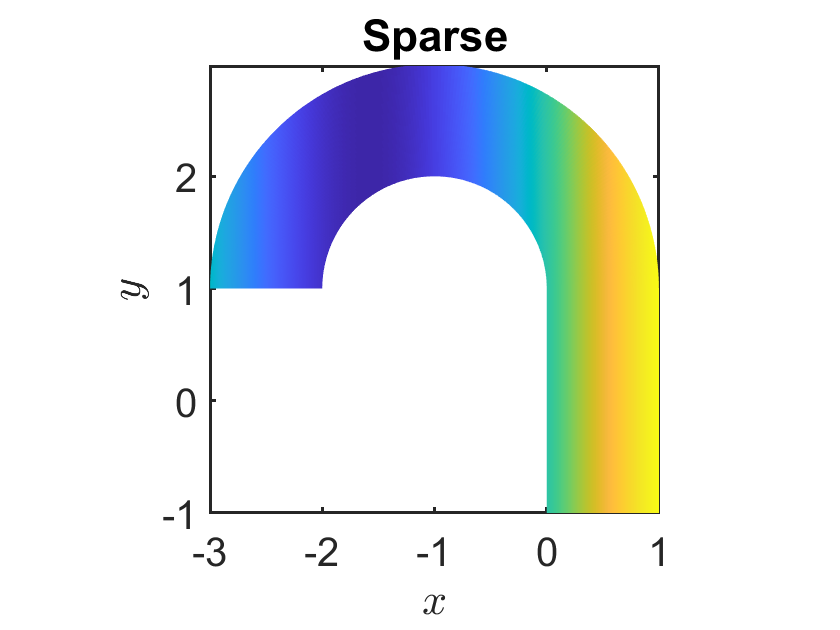
\includegraphics[scale=0.3]{Ex1a.png}
	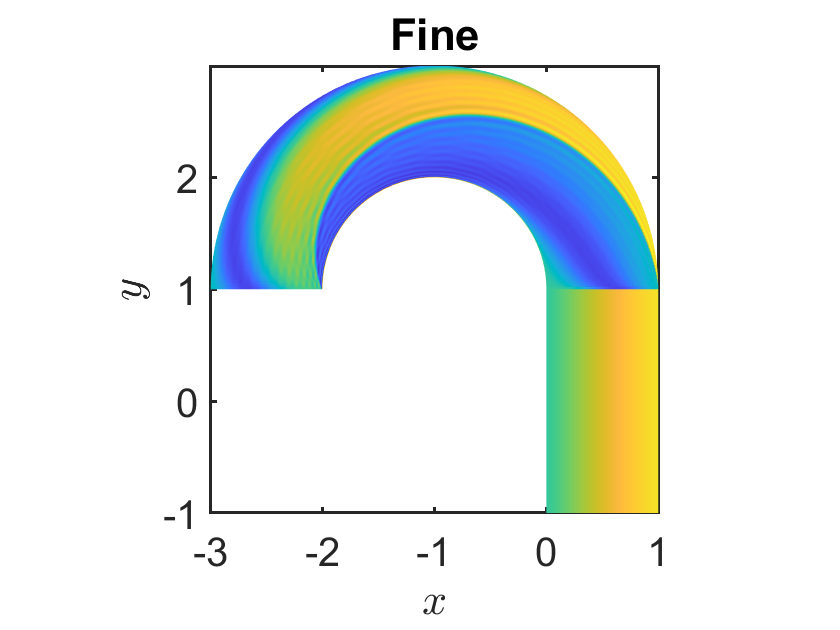
\includegraphics[scale=0.3]{Ex1b.png}
	\caption{Example 1} 
	\label{F1}
\end{figure} 	
\begin{figure}[h]
	\centering
	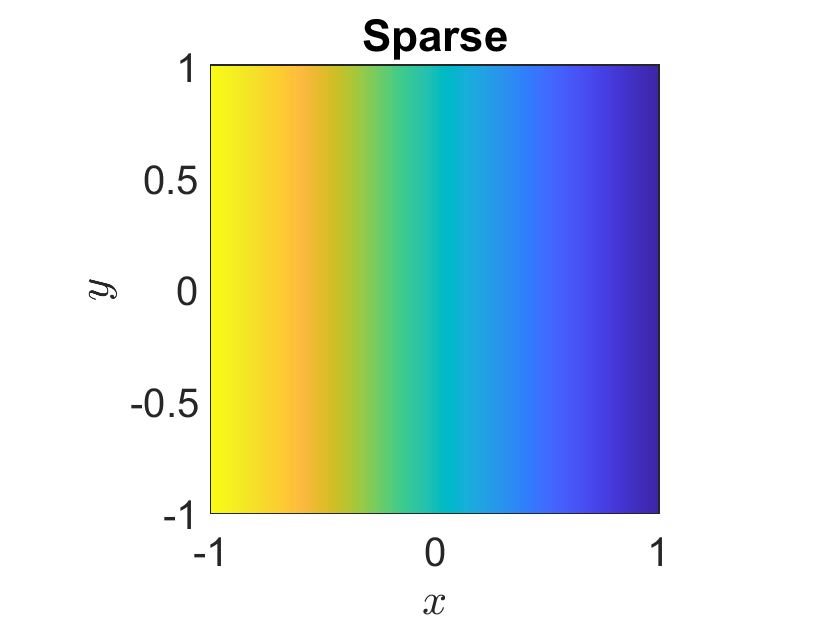
\includegraphics[scale=0.3]{Ex2a.png}
	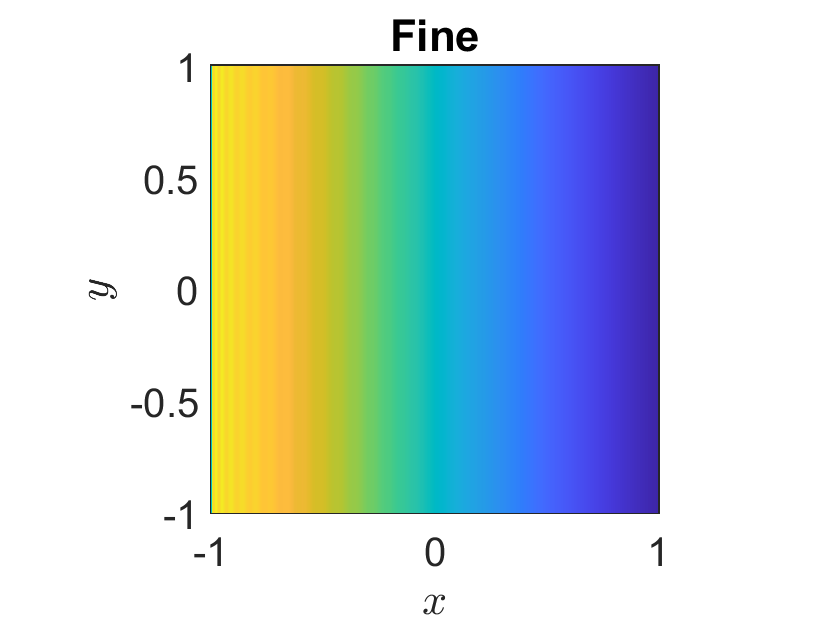
\includegraphics[scale=0.3]{Ex2b.png}
	\caption{Example 2} 
	\label{F2}
\end{figure} 
\begin{figure}[h]
	\centering
	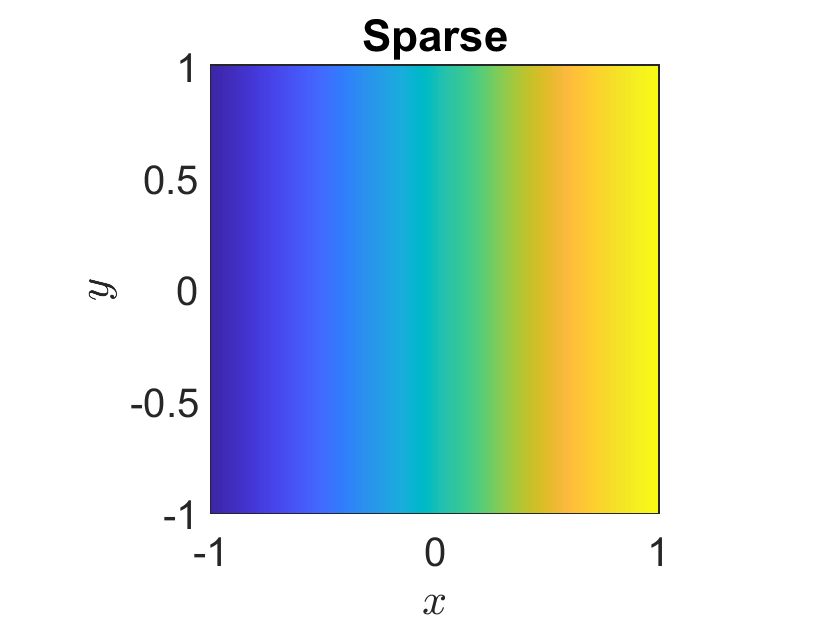
\includegraphics[scale=0.3]{Ex3a.png}
	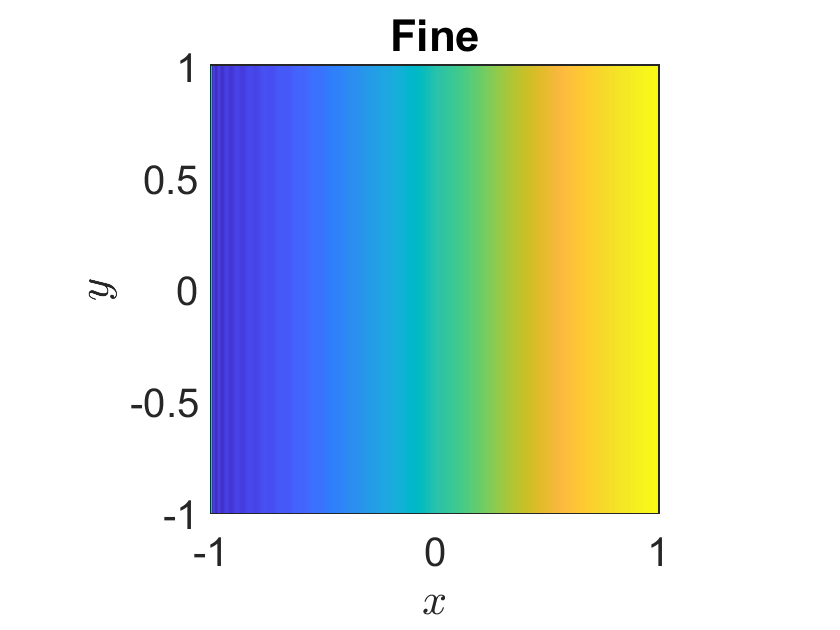
\includegraphics[scale=0.3]{Ex3b.png}
	\caption{Example 3} 
	\label{F3}
\end{figure} 	
\begin{figure}[h]
	\centering
	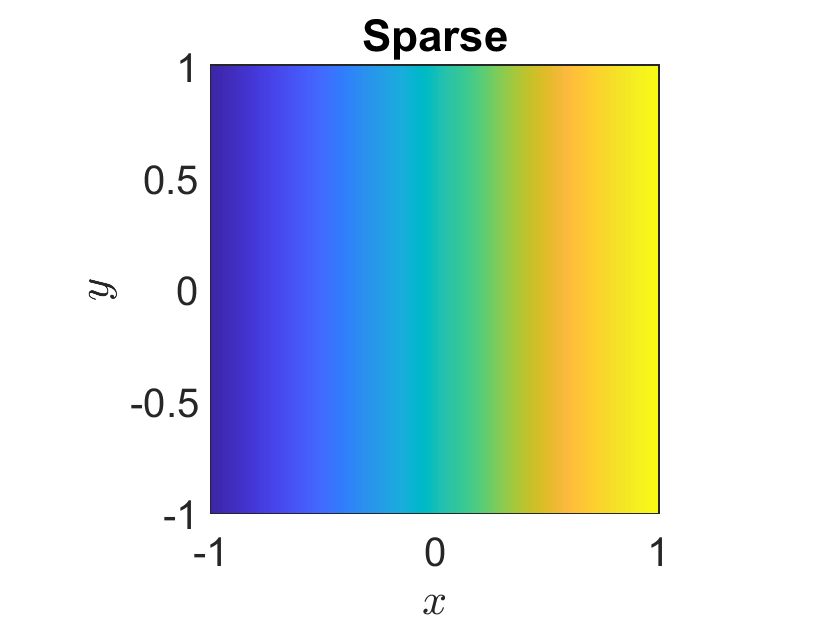
\includegraphics[scale=0.3]{Ex4a.png}
	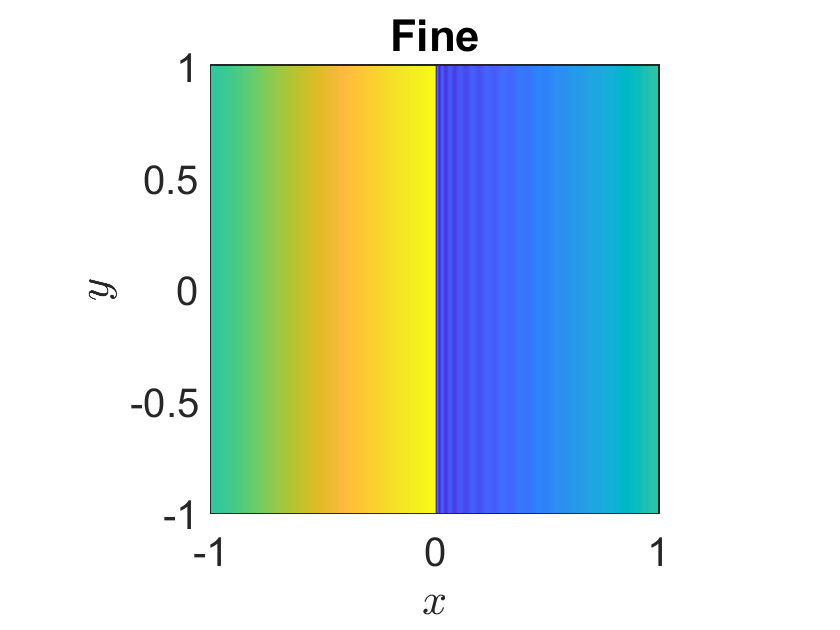
\includegraphics[scale=0.3]{Ex4b.png}
	\caption{Example 4} 
	\label{F4}
\end{figure} 	



\section{Sedimentation Paper}
	We have:
	\begin{align*}
	&\frac{\partial \rho}{\partial t} = \nabla \cdot \left( \Gamma \rho \nabla \frac{\delta F[\rho]}{\delta \rho} \right) \\
	&F[\rho] = k_BT \int \rho (\ln(\rho)  - 1)dr + \int \rho V_{ext} dr + F_{exc} [\rho],  
	\end{align*}
	with:
	\begin{align*}
	V_{ext} = \frac{k_BT z}{\xi}, \quad \xi = \frac{k_BT}{mg} \qquad \text{for} \quad \sigma/2 < z < L - \sigma /2.
	\end{align*}
	What's $\sigma$, the particle diameter, in our case?\\
	Then we have $\Gamma$, which is defined as:
	\begin{align*}
	&\Gamma_{HI} / \Gamma_0 = (1 - \phi^3)/ [ 1+ 2 \phi + 1.492 \phi(1-\phi^3)],\\
	& \phi = 4 \pi \rho a^3/3,
	\end{align*}
	where $a$ is the particle radius. 
	However, in the simulations we use the constant mobility, with overall packing fraction $\phi_0$:
	\begin{align*}
	\Gamma_{HI}(\phi_0), \quad \phi_0 = \pi \sigma^3 \nu / 6L.
	\end{align*}
	What is $\nu$ (the number density per area)? and do we have to scale the above formula by $\Gamma_0 = (6 \pi \mu a)^{-1}$ (which I am not sure is the right expression)?
	Overall, I think we could just implement the values they chose in their table. But their $F_{exc}$ will be different from ours, so I don't know whether that makes sense.
	The paper uses Rosenfeld's FMT.
	
	
	\section{Constriction Paper}
	We have:
	\begin{align*}
	&\frac{\partial \rho}{\partial t} = \nabla \cdot \left(  \rho \nabla \frac{\delta F[\rho]}{\delta \rho} \right) \\
	&F[\rho] = k_BT \int \rho (\ln(\rho)  - 1)dr + \int \rho( V_{ext} - fx) dr + F_{exc} [\rho], 
	\end{align*}
	where $f = k_BT/l$, $l$ is a unit length (interparticle distance).
	Further:
	\begin{align*}
	V_{ext} = V_0 [1 - 0.5erf((y+g(x))/\sqrt 2 w) + 0.5erf((y-g(x))/\sqrt 2 w)]
	\end{align*}
	\begin{align*}
	g(x) &= L_y /2 - \alpha [1+ \cos(2\pi (x - x_0)/L_c)] \quad \text{for} \quad |x - x_0| < L_c/2,\\
	&= L_y /2 \quad \text{otherwise}\\
	& \alpha = (L_y/4)(1-b),
	\end{align*}
	where $L_y$ is the channel height and $L_c$ is the constriction width, $b$ is the parameter that decides constriction height.\\
	Q: What is $w$? How do we find $l$? How do we know the number of particles in DDFT? Formula $\rho_0 = N/A_0 = 1/l^2$. \\
	Then we have $\Gamma = u_0 \rho_0^{3/2}/(k_BT)$, which is the measurement of interaction strength they use, so I need to know $\rho_0$.\\
	Question: The form of $F_{exc}[\rho]$ involves $c_0^{(2)}$, the pair direct correlation function, which is different from our implementation. \\
	Do we model in a box that's bigger or equal to $L_y$. 

	
	
	
	
	
	
	
	
	
\end{document}